\documentclass{article}

% Language setting
% Replace `english' with e.g. `spanish' to change the document language
\usepackage[english]{babel}

% Set page size and margins
% Replace `letterpaper' with`a4paper' for UK/EU standard size
\usepackage[letterpaper,top=2cm,bottom=2cm,left=3cm,right=3cm,marginparwidth=1.75cm]{geometry}

% Useful packages
\usepackage{amsmath}
\usepackage{graphicx}
\usepackage[colorlinks=true, allcolors=blue]{hyperref}

\title{EAFIT UNIVERSITY \\
    \large DEPARTMENT OF INFORMATICS AND SYSTEMS\\
     PROJECT CHOICE}
\author{Second Report}

\begin{document}
\maketitle

\section*{Course}
Numerical analysis
\section*{Teacher}
Edwar Samir Posada Murillo
\section*{Semester} 
2022-1
\section*{Project's name}
Numerical Algorithms
\section*{Repository}
This project has a GitHub repository where the evidence related with it will be. \url{https://github.com/DanielHernandezO/NumericalMethodsProject}
\section*{Members}
    \begin{enumerate}
        \item Jose Miguel Blanco Velez
        \item Neller Pellegrino Baquero
        \item Samuel David Villegas Bedoya
        \item Daniel Andres Hernandez Oyola
    \end{enumerate}
\section*{Project's description}
Webpage used to calculate data using different types of numerical methods with the option of visualising them in a 2d graph.
\section*{Added values}
    \begin{enumerate}
        \item The project will be done in english
        \item The project will have its documentation in latex
        \item The numerical algorithms can be found in multiple programming languages
        \item The project will have extra numerical methods
    \end{enumerate}

\begin{section}{Incremental Search - JavaScript}
   \textbf{Input data}\newline
    \[f(x)=ln(sin(x)^2+1)-(1/2)\]\newline
    x0 = -3\newline
    delta = 0.5\newline
    iterations = 100 \newline\newline
    \includegraphics[width=15cm]{Image/IncrementalSearchJavaScript.png}
\end{section}

\begin{section}{Incremental Search - Matlab}
   \textbf{Input data}\newline
    \[f(x)=ln(sin(x)^2+1)-(1/2)\]\newline
    x0 = -3\newline
    delta = 0.5\newline
    iterations = 100 \newline\newline
    \includegraphics[width=15cm]{Image/IncrementalSearchMatlab.png}
\end{section}
\begin{section}{Bisection - JavaScript}
   \textbf{Input data}\newline
    \[f(x)=ln(sin(x)^2+1)-(1/2)\]\newline
    a = 0\newline
    b=1 \newline
    Tolerance = 1e-7\newline
    iterations = 100 \newline\newline
    \includegraphics[width=15cm]{Image/BisectionJavaScript.png}
\end{section}
\begin{section}{Bisection - Matlab}
   \textbf{Input data}\newline
    \[f(x)=ln(sin(x)^2+1)-(1/2)\]\newline
    a = 0\newline
    b=1 \newline
    Tolerance = 1e-7\newline
    iterations = 100 \newline\newline
    \includegraphics[width=15cm]{Image/BisectionMatlab.png}
\end{section}
\begin{section}{Newton - JavaScript}
   \textbf{Input data}\newline
    \[f(x)=ln(sin(x)^2+1)-(1/2)\]\newline
    \[f'(x)=2(sin(x)^2+1)^-^1 sin(x)*cos(x)\]\newline
    x0=0.5 \newline
    Tolerance = 1e-7\newline
    iterations = 100 \newline\newline
    \includegraphics[width=15cm]{Image/NewtonJavaScript.png}
\end{section}
\begin{section}{Newton - Matlab}
   \textbf{Input data}\newline
    \[f(x)=ln(sin(x)^2+1)-(1/2)\]\newline
    \[f'(x)=2(sin(x)^2+1)^-^1 sin(x)*cos(x)\]\newline
    x0=0.5 \newline
    Tolerance = 1e-7\newline
    iterations = 100 \newline\newline
    \includegraphics[width=15cm]{Image/NewtonMatlab.png}
\end{section}
\begin{section}{Trisection - JavaScript}
   \textbf{Input data}\newline
    \[f(x)=ln(sin(x)^2+1)-(1/2)\]\newline
    a = 0\newline
    b=1 \newline
    Tolerance = 1e-7\newline
    iterations = 100 \newline\newline
    \includegraphics[width=15cm]{Image/TrisectionJavaScript.png}
\end{section}
\begin{section}{Trisection - Matlab}
   \textbf{Input data}\newline
    \[f(x)=ln(sin(x)^2+1)-(1/2)\]\newline
    a = 0\newline
    b=1 \newline
    Tolerance = 1e-7\newline
    iterations = 100 \newline\newline
    \includegraphics[width=15cm]{Image/TrisectionMatlab.png}
\end{section}
\begin{section}{Fixed Point - Javascript}
   \textbf{Input data}\newline
    \[log((sin(x)^2)+1)-x-1/2\]\newline
    \[log((sin(x)^2)+1)-1/2\]\newline
    x0 = -0.5\newline
    Tolerance = 10e-7\newline
    iterations = 100 \newline\newline
    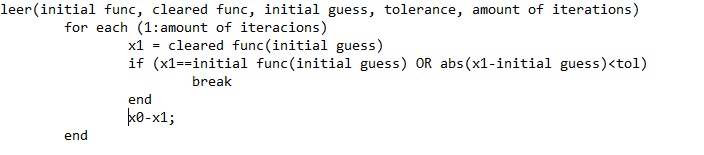
\includegraphics[width=15cm]{Image/fixedpoint.png}
\end{section}
\begin{section}{Fixed Point - Matlab}
   \textbf{Input data}\newline
    \[log((sin(x)^2)+1)-x-1/2\]\newline
    \[log((sin(x)^2)+1)-1/2\]\newline
    x0 = -0.5\newline
    Tolerance = 10e-7\newline
    iterations = 100 \newline\newline
    \includegraphics[width=5cm,height=15cm]{Image/fixedpointmatlab.png}
\end{section}
\begin{section}{gaussSimple - Javascript}
   \textbf{Input data}\newline
    \[A=\begin{pmatrix}
        2 & -1 & 0 & 3\\
        1 & 0.5 & 3 & 8\\
        0 & 13 & -2 & 11\\
        14 & 5 & -2 & 3
    \end{pmatrix}\]
    \[b=\begin{pmatrix}
        1\\
        1\\
        1\\
        1
    \end{pmatrix}\]
    n = 4\newline\newline
    \includegraphics[width=15cm,height=15cm]{Image/GaussSimple.PNG}
\end{section}
\begin{section}{gaussSimple - Matlab}
   \textbf{Input data}\newline
    \[A=\begin{pmatrix}
        2 & -1 & 0 & 3\\
        1 & 0.5 & 3 & 8\\
        0 & 13 & -2 & 11\\
        14 & 5 & -2 & 3
    \end{pmatrix}\]
    \[b=\begin{pmatrix}
        1\\
        1\\
        1\\
        1
    \end{pmatrix}\]
    n = 4\newline\newline
    \includegraphics[width=15cm,height=15cm]{Image/GaussSimpleMatlab.PNG}
\end{section}
\begin{section}{gaussPartialPivot - Javascript}
   \textbf{Input data}\newline
    \[A=\begin{pmatrix}
        2 & -1 & 0 & 3\\
        1 & 0.5 & 3 & 8\\
        0 & 13 & -2 & 11\\
        14 & 5 & -2 & 3
    \end{pmatrix}\]
    \[b=\begin{pmatrix}
        1\\
        1\\
        1\\
        1
    \end{pmatrix}\]
    n = 4\newline\newline
    \includegraphics[width=15cm,height=15cm]{Image/GaussPartialPivot.PNG}
\end{section}
\begin{section}{gaussPartialPivot - Matlab}
   \textbf{Input data}\newline
    \[A=\begin{pmatrix}
        2 & -1 & 0 & 3\\
        1 & 0.5 & 3 & 8\\
        0 & 13 & -2 & 11\\
        14 & 5 & -2 & 3
    \end{pmatrix}\]
    \[b=\begin{pmatrix}
        1\\
        1\\
        1\\
        1
    \end{pmatrix}\]
    n = 4\newline\newline
    \includegraphics[width=15cm,height=15cm]{Image/GaussPartialPivotMatlab.PNG}
\end{section}

\begin{section}{gaussTotalPivot - Javascript}
   \textbf{Input data}\newline
    \[A=\begin{pmatrix}
        2 & -1 & 0 & 3\\
        1 & 0.5 & 3 & 8\\
        0 & 13 & -2 & 11\\
        14 & 5 & -2 & 3
    \end{pmatrix}\]
    \[b=\begin{pmatrix}
        1\\
        1\\
        1\\
        1
    \end{pmatrix}\]
    n = 4\newline\newline
    \includegraphics[width=15cm,height=15cm]{Image/GaussTotalPivot.PNG}
\end{section}
\begin{section}{gaussTotalPivot - Matlab}
   \textbf{Input data}\newline
    \[A=\begin{pmatrix}
        2 & -1 & 0 & 3\\
        1 & 0.5 & 3 & 8\\
        0 & 13 & -2 & 11\\
        14 & 5 & -2 & 3
    \end{pmatrix}\]
    \[b=\begin{pmatrix}
        1\\
        1\\
        1\\
        1
    \end{pmatrix}\]
    n = 4\newline\newline
    \includegraphics[width=15cm,height=15cm]{Image/GaussTotalPivotMatlab.PNG}
\end{section}

\begin{section}{multiple roots - Javascript}
   \textbf{Input data}\newline
    \[h(x) = e^x-x-1\]\newline
    \[h'(x) = e^x-1\]\newline
     \[h''(x)= e^x\]\newline
    x0 = 1\newline
    Tolerance = 10e-7\newline
    iterations = 100 \newline\newline
    \includegraphics[width=15cm]{Image/MultipleRoot.PNG}
\end{section}
\begin{section}{multiple roots - Matlab}
   \textbf{Input data}\newline
    \[h(x) = e^x-x-1\]\newline
    \[h'(x) = e^x-1\]\newline
     \[h''(x)= e^x\]\newline
    x0 = 1\newline
    Tolerance = 10e-7\newline
    iterations = 100 \newline\newline
    \includegraphics[width=15cm,height=15cm]{Image/MultipleRootMatlab.PNG}
\end{section}

\begin{section}{Aitken - Javascript}
   \textbf{Input data}\newline
    \[f_{1}(x) = log((sin(x)^2)+1)-x-1/2\]\newline
    \[g(x) = log((sin(x)^2)+1)-1/2\]\newline
    x0 = -0.5\newline
    Tolerance = 10e-7\newline
    iterations = 100 \newline\newline
    \includegraphics[width=15cm]{Image/Aitken.PNG}
\end{section}
\begin{section}{Aitken - Matlab}
   \textbf{Input data}\newline
    \[f_{1}(x) = log((sin(x)^2)+1)-x-1/2\]\newline
    \[g(x) = log((sin(x)^2)+1)-1/2\]\newline
    x0 = -0.5\newline
    Tolerance = 10e-7\newline
    iterations = 100 \newline\newline
    \includegraphics[width=20cm,height=15cm]{Image/AitkenMatlab.PNG}
\end{section}


\begin{section}{steffensen - Javascript}
   \textbf{Input data}\newline
   \[f_{1}(x) = log((sin(x)^2)+1)-x-1/2\]\newline
    \[g(x) = log((sin(x)^2)+1)-1/2\]\newline
    x0 = -0.5\newline
    Tolerance = 10e-7\newline
    iterations = 100 \newline\newline
    \includegraphics[width=15cm]{Image/Steffensen.PNG}
\end{section}
\begin{section}{steffensen - Matlab}
   \textbf{Input data}\newline
    \[f_{1}(x) = log((sin(x)^2)+1)-x-1/2\]\newline
    \[g(x) = log((sin(x)^2)+1)-1/2\]\newline
    x0 = -0.5\newline
    Tolerance = 10e-7\newline
    iterations = 100 \newline\newline
    \includegraphics[width=15cm,height=15cm]{Image/SteffensenMatlab.PNG}
\end{section}

\begin{section}{muller - Javascript}
   \textbf{Input data}\newline
   \[f(x)=ln(sin(x)^2+1)-(1/2)\]\newline
    x0 = 0.5\newline
    x1 = 1\newline
    Tolerance = 10e-7\newline
    iterations = 100 \newline\newline
    \includegraphics[width=15cm]{Image/Muller.PNG}
\end{section}
\begin{section}{muller - Matlab}
   \textbf{Input data}\newline
    \[f(x)=ln(sin(x)^2+1)-(1/2)\]\newline
    x0 = 0.5\newline
    x1 = 1\newline
    Tolerance = 10e-7\newline
    iterations = 100 \newline\newline
    \includegraphics[width=15cm,height=15cm]{Image/MullerMatlab.PNG}
\end{section}
\begin{section}{secant method - Mathlab}
   \textbf{Input data}\newline
    \[log((sin(x)^2)+1)-x-1/2\]\newline
    \[log((sin(x)^2)+1)-1/2\]\newline
    x0 = 0.5\newline
    x1 = 1\newline
    Tolerance = 10e-7\newline
    iterations = 100 \newline\newline
    \includegraphics[width=15cm]{Image/pruebasecante.PNG}
\end{section}
\begin{section}{secant method - JavaScript}
   \textbf{Input data}\newline
    \[log((sin(x)^2)+1)-x-1/2\]\newline
    \[log((sin(x)^2)+1)-1/2\]\newline
    x0 = 0.5\newline
    x1 = 1\newline
    Tolerance = 10e-7\newline
    iterations = 100 \newline\newline
    \includegraphics[width=15cm]{Image/pruebasecantejs.png}
\end{section}
\begin{section}{false position - Mathlab}
   \textbf{Input data}\newline
    \[log((sin(x)^2)+1)-x-1/2\]\newline
    \[log((sin(x)^2)+1)-1/2\]\newline
    a = 0\newline
    b = 1\newline
    Tolerance = 10e-7\newline
    iterations = 100 \newline\newline
    \includegraphics[width=15cm]{Image/pruebareglafalse.PNG}
\end{section}
\begin{section}{false position - JavaScript}
   \textbf{Input data}\newline
    \[log((sin(x)^2)+1)-x-1/2\]\newline
    \[log((sin(x)^2)+1)-1/2\]\newline
    a = 0\newline
    b = 1\newline
    Tolerance = 10e-7\newline
    iterations = 100 \newline\newline
    \includegraphics[width=15cm]{Image/pruebareglafalsejs.png}
\end{section}
\begin{section}{gaussian elimination for tridiagonal matrices - Mathlab}
   \textbf{Input data}\newline
   a = [0,3,2,1]\newline
   b = [1,4,3,3]\newline
   c = [4,1,4,0]\newline
   d = [1,1,1,1]\newline
    \includegraphics[width=15cm]{Image/TDMAPrueba.PNG}
\end{section}
\begin{section}{gaussian elimination for tridiagonal matrices-JavaScript}
   \textbf{Input data}\newline
   a = [0,3,2,1]\newline
   b = [1,4,3,3]\newline
   c = [4,1,4,0]\newline
   d = [1,1,1,1]\newline
    \includegraphics[width=15cm]{Image/pruebatdma.jpeg}
\end{section}

\section*{Members signatures}
Jose Miguel \\
Daniel Hernandez \\
Neller Pellegrino \\
Samuel Villegas \\
\end{document}